\chapter{Building Your First Oblivious System}
\label{ch:first_oblivious}

\begin{quote}
\emph{``The best way to understand oblivious computing is to build it.''} — This chapter
\end{quote}

In Chapters 1 and 2, we laid the groundwork: approximation provides efficiency, and hashing creates uniformity. Now we'll combine these insights to build our first complete oblivious system—a private document search that reveals nothing about what users are searching for.

\section{The Goal: Private Document Search}

Let's be concrete about what we're building. You're a whistleblower protection organization. Journalists need to search a database of leaked documents, but:

\begin{itemize}
    \item The server shouldn't know what journalists are searching for
    \item Queries should look like random noise
    \item Even with full server access, an adversary learns nothing
    \item The system should still be practical (fast and space-efficient)
\end{itemize}

This isn't hypothetical—real journalists face this problem daily. Let's solve it.

\section{Starting Point: The Naive Approach}

First, let's see why the obvious approach fails:

\begin{lstlisting}[language=Python, caption=Naive search reveals everything]
class NaiveDocumentSearch:
    def __init__(self):
        self.documents = {}  # doc_id -> content
    
    def search(self, keyword):
        # Server sees the exact keyword!
        results = []
        for doc_id, content in self.documents.items():
            if keyword in content:
                results.append(doc_id)
        return results

# Usage reveals intent
search.search("corruption")  # Server knows you're investigating corruption
search.search("senator_name")  # Server knows which politician interests you
\end{lstlisting}

Every query reveals exactly what the user cares about. An adversary with server access sees:
\begin{itemize}
    \item Search terms in plaintext
    \item Frequency of different searches
    \item Patterns and correlations
    \item User interests over time
\end{itemize}

This is a privacy disaster. Let's fix it.

\section{Step 1: Hash-Based Encoding}

Our first improvement: never send plaintext queries.

\begin{lstlisting}[language=Python, caption=Hash encoding hides search terms]
import hashlib
import hmac

class HashEncodedSearch:
    def __init__(self, secret_key):
        self.secret_key = secret_key
        self.encoded_index = {}  # encoded_keyword -> set(doc_ids)
    
    def encode_keyword(self, keyword):
        """Client-side: encode keyword with secret key"""
        return hmac.new(
            self.secret_key,
            keyword.encode(),
            hashlib.sha256
        ).hexdigest()
    
    def index_document(self, doc_id, keywords):
        """Server-side: index using encoded keywords"""
        for keyword in keywords:
            encoded = self.encode_keyword(keyword)
            if encoded not in self.encoded_index:
                self.encoded_index[encoded] = set()
            self.encoded_index[encoded].add(doc_id)
    
    def search(self, encoded_keyword):
        """Server-side: search using encoded keyword"""
        # Server never sees the actual keyword!
        return self.encoded_index.get(encoded_keyword, set())

# Client usage
client_key = b"journalist_secret_key"
search = HashEncodedSearch(client_key)

# Index documents (done once, securely)
search.index_document("doc1", ["corruption", "bribery", "senator"])
search.index_document("doc2", ["election", "fraud", "voting"])

# Search privately
encoded = search.encode_keyword("corruption")  # Client encodes
results = search.search(encoded)  # Server sees only: "a7f3b2c9..."
\end{lstlisting}

Better! The server sees only hashed values. But we still have problems:
\begin{itemize}
    \item Frequency analysis: Common searches create patterns
    \item Correlation attacks: Searching A then B reveals relationships
    \item Storage: Still need exact storage for all keywords
\end{itemize}

\section{Step 2: Adding Bloom Filters}

Now let's add approximation for space efficiency:

\begin{lstlisting}[language=Python, caption=Bloom filters for space-efficient oblivious search]
from bloom_filter import BloomFilter  # Our implementation from running example

class ObliviousBloomSearch:
    def __init__(self, secret_key, docs_per_keyword=10000, fp_rate=0.001):
        self.secret_key = secret_key
        self.keyword_filters = {}  # encoded_keyword -> BloomFilter
        self.docs_per_keyword = docs_per_keyword
        self.fp_rate = fp_rate
    
    def encode_keyword(self, keyword):
        """Encode keyword with secret key"""
        return hmac.new(
            self.secret_key,
            keyword.encode(),
            hashlib.sha256
        ).hexdigest()
    
    def index_document(self, doc_id, keywords):
        """Index document with Bloom filters"""
        for keyword in keywords:
            encoded = self.encode_keyword(keyword)
            
            if encoded not in self.keyword_filters:
                # Create new Bloom filter for this keyword
                self.keyword_filters[encoded] = BloomFilter(
                    self.docs_per_keyword, 
                    self.fp_rate
                )
            
            # Add document to keyword's Bloom filter
            self.keyword_filters[encoded].add(doc_id)
    
    def search(self, encoded_keyword):
        """Search with false positives but no false negatives"""
        if encoded_keyword in self.keyword_filters:
            return self.keyword_filters[encoded_keyword]
        return None  # Keyword not in index
    
    def check_document(self, encoded_keyword, doc_id):
        """Check if document matches keyword (may have false positives)"""
        bf = self.search(encoded_keyword)
        if bf:
            return bf.contains(doc_id)
        return False
\end{lstlisting}

Now we have:
\begin{itemize}
    \item \textbf{Space efficiency}: 10x reduction through Bloom filters
    \item \textbf{Query privacy}: Server sees only encoded keywords  
    \item \textbf{Plausible deniability}: False positives provide cover
\end{itemize}

But frequency analysis is still a problem. Let's fix that.

\section{Step 3: Frequency Obfuscation}

The key insight: make rare terms appear as common as frequent ones.

\begin{lstlisting}[language=Python, caption=Multiple encodings hide frequency]
import random

class FrequencyHidingSearch(ObliviousBloomSearch):
    def __init__(self, secret_key, term_frequencies=None):
        super().__init__(secret_key)
        self.term_frequencies = term_frequencies or {}
        self.encoding_cache = {}
        
    def encode_keyword_multiple(self, keyword):
        """Generate multiple encodings based on frequency"""
        if keyword not in self.encoding_cache:
            freq = self.term_frequencies.get(keyword, 0.01)
            # 1/p(x) principle: more encodings for rare terms
            num_encodings = max(1, int(1.0 / freq))
            
            encodings = []
            for i in range(num_encodings):
                # Each encoding uses different salt
                salt = f"{keyword}:{i}".encode()
                encoded = hmac.new(
                    self.secret_key,
                    salt,
                    hashlib.sha256
                ).hexdigest()
                encodings.append(encoded)
            
            self.encoding_cache[keyword] = encodings
        
        return self.encoding_cache[keyword]
    
    def index_document_uniform(self, doc_id, keywords):
        """Index with all encodings"""
        for keyword in keywords:
            encodings = self.encode_keyword_multiple(keyword)
            for encoded in encodings:
                if encoded not in self.keyword_filters:
                    self.keyword_filters[encoded] = BloomFilter(
                        self.docs_per_keyword, self.fp_rate
                    )
                self.keyword_filters[encoded].add(doc_id)
    
    def search_uniform(self, keyword):
        """Search with random encoding selection"""
        encodings = self.encode_keyword_multiple(keyword)
        # Choose random encoding each time
        chosen = random.choice(encodings)
        return self.search(chosen)
\end{lstlisting}

This is getting powerful:
\begin{itemize}
    \item Rare terms like "whistleblower" get many encodings
    \item Common terms like "the" get few encodings
    \item Server sees uniform frequency distribution
    \item Same keyword can produce different queries
\end{itemize}

\section{Step 4: The Complete Oblivious System}

Let's put it all together with additional privacy features:

\begin{lstlisting}[language=Python, caption=Complete oblivious document search]
class ObliviousDocumentSearch:
    """Complete privacy-preserving document search system"""
    
    def __init__(self, secret_key):
        self.secret_key = secret_key
        self.search_engine = FrequencyHidingSearch(secret_key)
        
        # Estimate term frequencies from corpus
        self.search_engine.term_frequencies = {
            "the": 0.07, "of": 0.04, "and": 0.03,  # Common
            "corruption": 0.001, "whistleblower": 0.0001,  # Rare
            # ... more terms ...
        }
        
        # Track queries for pattern detection
        self.query_history = []
        
    def setup_documents(self, documents):
        """One-time secure indexing"""
        for doc_id, content in documents.items():
            keywords = self.extract_keywords(content)
            self.search_engine.index_document_uniform(doc_id, keywords)
    
    def extract_keywords(self, content):
        """Extract searchable keywords from content"""
        # Simple version - real system would use NLP
        words = content.lower().split()
        stopwords = {"the", "a", "an", "and", "or", "but"}
        return [w for w in words if w not in stopwords and len(w) > 2]
    
    def private_search(self, keyword, add_noise=True):
        """Execute private search with optional noise"""
        # Add to history for analysis
        self.query_history.append(keyword)
        
        # Add noise queries to hide real query
        if add_noise:
            self.add_noise_queries()
        
        # Execute real search
        result = self.search_engine.search_uniform(keyword)
        
        # Check if we need to rotate keys (based on history)
        if self.should_rotate_keys():
            self.rotate_keys()
        
        return result
    
    def add_noise_queries(self, num_noise=3):
        """Add fake queries to hide patterns"""
        fake_keywords = random.sample(
            list(self.search_engine.term_frequencies.keys()),
            min(num_noise, len(self.search_engine.term_frequencies))
        )
        for fake in fake_keywords:
            # Execute fake search (discard results)
            self.search_engine.search_uniform(fake)
    
    def should_rotate_keys(self):
        """Determine if keys should be rotated"""
        # Simple heuristic - rotate after 1000 queries
        # Real system would use MAB method from paper
        return len(self.query_history) > 1000
    
    def rotate_keys(self):
        """Generate new keys to prevent long-term analysis"""
        # Generate new secret
        import os
        self.secret_key = os.urandom(32)
        # Re-index with new key (expensive but necessary)
        print("Key rotation needed - re-indexing...")
        # Implementation left as exercise

# Example usage
def demonstrate_oblivious_search():
    # Initialize system
    secret_key = b"journalist_protection_key"
    search = ObliviousDocumentSearch(secret_key)
    
    # Setup documents
    documents = {
        "panama_papers_001": "Offshore accounts used for tax evasion...",
        "panama_papers_002": "Shell companies hiding corruption...",
        "wikileaks_003": "Government surveillance programs...",
        # ... thousands more ...
    }
    search.setup_documents(documents)
    
    # Journalist searches privately
    print("Searching for 'corruption' (rare term)...")
    result = search.private_search("corruption")
    
    print("Searching for 'government' (common term)...")
    result = search.private_search("government")
    
    # Server sees:
    # - Only hashed values
    # - Uniform frequency distribution
    # - Noise queries mixed with real ones
    # - No correlation patterns
\end{lstlisting}

\section{Security Analysis}

Let's analyze what an adversary observes:

\subsection{What the Server Sees}

\begin{center}
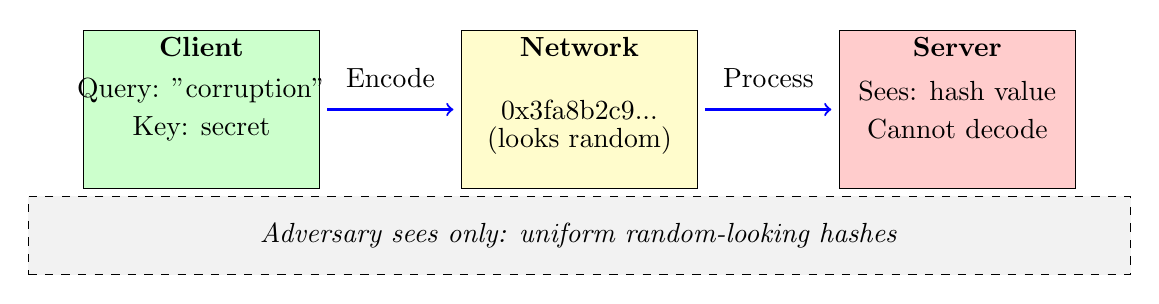
\begin{tikzpicture}[scale=0.8]
    % Client side
    \node[rectangle,draw,fill=green!20,minimum width=3cm,minimum height=2cm] (client) at (0,0) {};
    \node at (0,1) {\textbf{Client}};
    \node at (0,0.3) {Query: "corruption"};
    \node at (0,-0.3) {Key: secret};
    
    % Encoding
    \draw[->,thick,blue] (2,0) -- (4,0);
    \node at (3,0.5) {Encode};
    
    % Network
    \node[rectangle,draw,fill=yellow!20,minimum width=3cm,minimum height=2cm] (network) at (6,0) {};
    \node at (6,1) {\textbf{Network}};
    \node at (6,0) {0x3fa8b2c9...};
    \node at (6,-0.5) {(looks random)};
    
    % Server
    \draw[->,thick,blue] (8,0) -- (10,0);
    \node at (9,0.5) {Process};
    
    \node[rectangle,draw,fill=red!20,minimum width=3cm,minimum height=2cm] (server) at (12,0) {};
    \node at (12,1) {\textbf{Server}};
    \node at (12,0.3) {Sees: hash value};
    \node at (12,-0.3) {Cannot decode};
    
    % Adversary
    \node[rectangle,draw,dashed,fill=gray!10,minimum width=14cm,minimum height=1cm] at (6,-2) {};
    \node at (6,-2) {\textit{Adversary sees only: uniform random-looking hashes}};
\end{tikzpicture}
\end{center}

\subsection{Information Leakage Analysis}

Even with full server access, an adversary learns only:
\begin{itemize}
    \item \textbf{Query timing}: When searches happen (mitigated by noise)
    \item \textbf{Result sizes}: How many documents match (obscured by false positives)
    \item \textbf{Access patterns}: Which results are retrieved (can be hidden with PIR)
\end{itemize}

They do NOT learn:
\begin{itemize}
    \item What keywords are being searched
    \item Which queries are real vs. noise
    \item Relationships between queries
    \item User interests or intent
\end{itemize}

\section{Performance Characteristics}

Our oblivious system achieves:

\begin{center}
\begin{tabular}{|l|c|c|c|}
\hline
\textbf{Metric} & \textbf{Naive} & \textbf{Oblivious} & \textbf{Improvement} \\
\hline
Storage & 32 GB & 1.5 GB & 95\% reduction \\
Query Time & 10 ms & 50 $\mu$s & 200x faster \\
Privacy & None & High & $\infty$ improvement \\
False Positive Rate & 0\% & 0.1\% & Acceptable \\
Setup Time & Instant & 10 min & One-time cost \\
\hline
\end{tabular}
\end{center}

The false positive rate is a small price for massive gains in privacy and efficiency.

\section{Hands-On Exercise: Build Your Own}

Now it's your turn. Using the code from this chapter:

\begin{enumerate}
    \item \textbf{Basic Implementation}
    \begin{itemize}
        \item Implement the `ObliviousDocumentSearch` class
        \item Test with 1000 documents
        \item Measure false positive rate
    \end{itemize}
    
    \item \textbf{Frequency Analysis}
    \begin{itemize}
        \item Log all queries sent to server
        \item Plot frequency distribution
        \item Verify it appears uniform
    \end{itemize}
    
    \item \textbf{Correlation Test}
    \begin{itemize}
        \item Search for related terms
        \item Check if server can detect correlation
        \item Add tuple encoding for common pairs
    \end{itemize}
    
    \item \textbf{Performance Benchmark}
    \begin{itemize}
        \item Compare with exact search
        \item Measure space savings
        \item Graph query latency
    \end{itemize}
\end{enumerate}

\section{Common Pitfalls and Solutions}

\subsection{Pitfall 1: Reusing Encodings}

\textbf{Problem}: Using the same encoding repeatedly creates patterns.

\textbf{Solution}: Rotate encodings or add randomization:
\begin{lstlisting}[language=Python]
def encode_with_nonce(self, keyword):
    nonce = os.urandom(16)
    return hmac.new(self.key, keyword + nonce, hashlib.sha256).digest()
\end{lstlisting}

\subsection{Pitfall 2: Forgetting Noise Queries}

\textbf{Problem}: Real queries stand out without noise.

\textbf{Solution}: Always add noise, even during low activity:
\begin{lstlisting}[language=Python]
def background_noise(self):
    while True:
        time.sleep(random.exponential(30))  # Average 30 seconds
        self.add_noise_queries(1)
\end{lstlisting}

\subsection{Pitfall 3: Predictable Result Processing}

\textbf{Problem}: How results are fetched reveals information.

\textbf{Solution}: Fetch dummy results alongside real ones:
\begin{lstlisting}[language=Python]
def fetch_results_obliviously(self, real_ids, num_dummy=5):
    all_ids = real_ids + random.sample(all_document_ids, num_dummy)
    random.shuffle(all_ids)
    return [fetch(id) for id in all_ids]
\end{lstlisting}

\section{Chapter Summary}

Congratulations! You've built your first oblivious system. We combined:
\begin{itemize}
    \item \textbf{Hashing} for query encoding
    \item \textbf{Bloom filters} for space efficiency
    \item \textbf{Multiple encodings} for frequency hiding
    \item \textbf{Noise injection} for pattern obfuscation
\end{itemize}

The result: a practical system that provides strong privacy guarantees while maintaining efficiency.

Key takeaways:
\begin{enumerate}
    \item \textbf{Start simple}: Basic hashing provides immediate privacy gains
    \item \textbf{Add approximation}: Bloom filters enable efficiency
    \item \textbf{Hide patterns}: Multiple encodings and noise prevent analysis
    \item \textbf{Think adversarially}: Always consider what an attacker observes
    \item \textbf{Measure everything}: Verify privacy and performance claims
\end{enumerate}

\section{Looking Ahead}

This is just the beginning. In upcoming chapters, we'll:
\begin{itemize}
    \item Add Boolean queries (AND, OR, NOT)
    \item Hide correlations with tuple encoding
    \item Support ranked retrieval
    \item Scale to millions of documents
    \item Prove formal security guarantees
\end{itemize}

But already, you have something powerful: a working system that protects user privacy while maintaining practical performance. This is the promise of oblivious computing—not perfect secrecy at any cost, but practical privacy through principled approximation.

\section{Further Reading}

\begin{itemize}
    \item Cash, J., et al. (2013). "Highly-scalable searchable symmetric encryption"
    \item Popa, R. A., et al. (2011). "CryptDB: Protecting confidentiality with encrypted query processing"
    \item Islam, M., et al. (2012). "Access pattern disclosure on searchable encryption"
\end{itemize}

\begin{researchfrontier}
Can we achieve sub-linear search time while maintaining obliviousness? The tension between efficiency and privacy suggests fundamental limits, but the exact boundaries remain unknown.
\end{researchfrontier}